\documentclass[11pt]{standalone}
\usepackage{mathpazo}\usepackage[T1]{fontenc}\usepackage[utf8]{inputenc}
\usepackage{amsmath,amssymb}
\usepackage{tikz}
\usepackage{xcolor}
\usetikzlibrary{arrows.meta,positioning,calc,fit,backgrounds}

\definecolor{ink}{HTML}{16211E}
\definecolor{pine}{HTML}{1E5B4F}
\definecolor{mulberry}{HTML}{8C3A56}
\definecolor{slate}{HTML}{54655F}
\definecolor{rulec}{HTML}{B9C7C2}
\definecolor{boxbg}{HTML}{F5F8F7}
\definecolor{srcbg}{HTML}{EDF2F0}
\definecolor{evalbg}{HTML}{FBF6F7}

\newcommand{\ttl}{\sffamily\small\bfseries\color{pine}}
\newcommand{\frm}{\scriptsize\color{ink}}
\newcommand{\nte}{\scriptsize\color{slate}}
\begin{document}
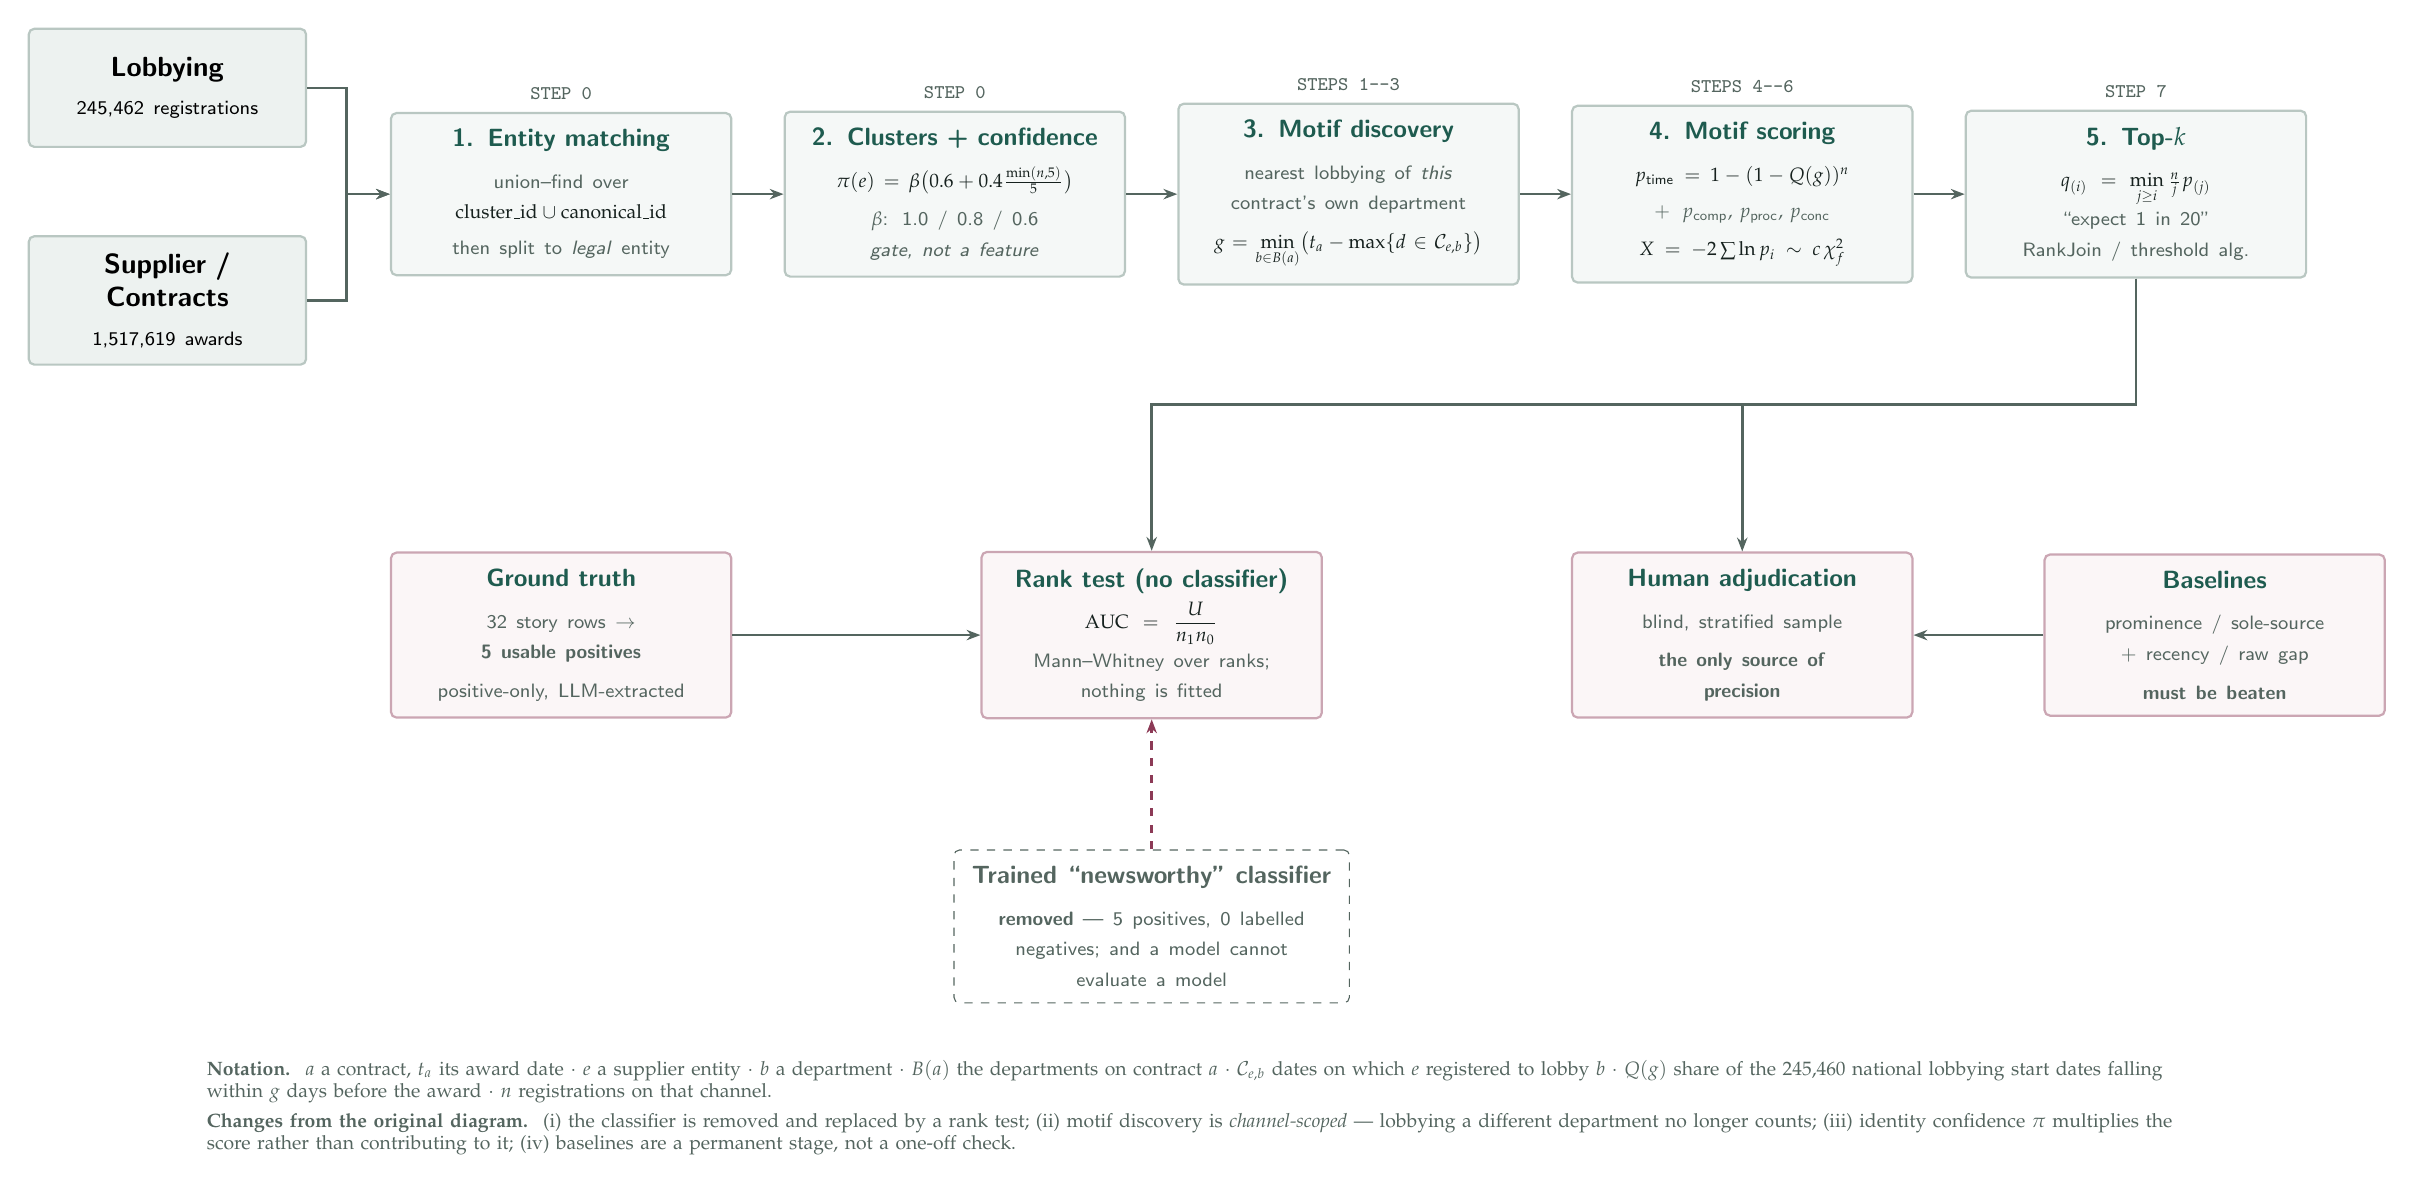
\begin{tikzpicture}[
  font=\sffamily,
  box/.style   ={draw=rulec, fill=boxbg, rounded corners=2pt, line width=0.8pt,
                 text width=3.9cm, align=center, inner sep=6pt, minimum height=1.9cm},
  src/.style   ={box, fill=srcbg, text width=3.1cm, minimum height=1.5cm},
  evl/.style   ={box, fill=evalbg, draw=mulberry!45},
  capt/.style  ={font=\scriptsize, color=slate},
  ar/.style    ={-{Stealth[length=5pt]}, draw=slate, line width=0.9pt},
  arx/.style   ={-{Stealth[length=5pt]}, draw=mulberry, line width=0.9pt, dashed},
  stg/.style  ={font=\ttfamily\scriptsize, color=slate}
]

%============================== ROW 1 : the scored path
\node[src] (lob) at (0,1.35)
  {\textbf{Lobbying}\\[2pt]{\scriptsize 245{,}462 registrations}};
\node[src] (sup) at (0,-1.35)
  {\textbf{Supplier / Contracts}\\[2pt]{\scriptsize 1{,}517{,}619 awards}};

\node[box] (em) at (5.0,0)
  {{\ttl 1. Entity matching}\\[3pt]
   {\nte union--find over}\\[-1pt]
   {\frm $\mathrm{cluster\_id}\cup\mathrm{canonical\_id}$}\\[1pt]
   {\nte then split to \emph{legal} entity}};

\node[box] (cl) at (10.0,0)
  {{\ttl 2. Clusters + confidence}\\[3pt]
   {\frm $\pi(e)=\beta\bigl(0.6+0.4\tfrac{\min(n,5)}{5}\bigr)$}\\[2pt]
   {\nte $\beta$: 1.0 / 0.8 / 0.6}\\[-1pt]
   {\nte \emph{gate, not a feature}}};

\node[box] (mot) at (15.0,0)
  {{\ttl 3. Motif discovery}\\[3pt]
   {\nte nearest lobbying of \emph{this}}\\[-1pt]
   {\nte contract's own department}\\[2pt]
   {\frm $g=\min\limits_{b\in B(a)}\bigl(t_a-\max\{d\in\mathcal{C}_{e,b}\}\bigr)$}};

\node[box] (sc) at (20.0,0)
  {{\ttl 4. Motif scoring}\\[3pt]
   {\frm $p_{\text{time}}=1-(1-Q(g))^{n}$}\\[1pt]
   {\nte $+\;p_{\text{comp}},\,p_{\text{proc}},\,p_{\text{conc}}$}\\[2pt]
   {\frm $X=-2\textstyle\sum\ln p_i \sim c\,\chi^2_f$}};

\node[box] (tk) at (25.0,0)
  {{\ttl 5. Top-$k$}\\[3pt]
   {\frm $q_{(i)}=\min\limits_{j\ge i}\tfrac{n}{j}p_{(j)}$}\\[2pt]
   {\nte ``expect 1 in 20''}\\[-1pt]
   {\nte RankJoin / threshold alg.}};

\draw[ar] (lob.east) -- ++(0.5,0) |- (em.west);
\draw[ar] (sup.east) -- ++(0.5,0) |- (em.west);
\draw[ar] (em)  -- (cl);
\draw[ar] (cl)  -- (mot);
\draw[ar] (mot) -- (sc);
\draw[ar] (sc)  -- (tk);

\node[stg, above=1pt of em]  {STEP 0};
\node[stg, above=1pt of cl]  {STEP 0};
\node[stg, above=1pt of mot] {STEPS 1--3};
\node[stg, above=1pt of sc]  {STEPS 4--6};
\node[stg, above=1pt of tk]  {STEP 7};

%============================== ROW 2 : evaluation
\node[evl] (gt) at (5.0,-5.6)
  {{\ttl Ground truth}\\[3pt]
   {\nte 32 story rows $\rightarrow$}\\[-1pt]
   {\nte \textbf{5 usable positives}}\\[2pt]
   {\nte positive-only, LLM-extracted}};

\node[evl] (rt) at (12.5,-5.6)
  {{\ttl Rank test \emph{(no classifier)}}\\[3pt]
   {\frm $\mathrm{AUC}=\dfrac{U}{n_1 n_0}$}\\[2pt]
   {\nte Mann--Whitney over ranks;}\\[-1pt]
   {\nte nothing is fitted}};

\node[evl] (hu) at (20.0,-5.6)
  {{\ttl Human adjudication}\\[3pt]
   {\nte blind, stratified sample}\\[2pt]
   {\nte \textbf{the only source of}}\\[-1pt]
   {\nte \textbf{precision}}};

\node[evl] (bl) at (26.0,-5.6)
  {{\ttl Baselines}\\[3pt]
   {\nte prominence / sole-source}\\[-1pt]
   {\nte $+$ recency / raw gap}\\[2pt]
   {\nte \textbf{must be beaten}}};

\draw[ar] (gt) -- (rt);
\draw[ar] (tk.south) -- ++(0,-1.6) -| (rt.north);
\draw[ar] (tk.south) -- ++(0,-1.6) -| (hu.north);
\draw[ar] (bl) -- (hu);

%============================== the removed box
\node[draw=slate!45, dashed, rounded corners=2pt, text width=4.6cm, align=center,
      inner sep=6pt, font=\sffamily, color=slate] (rm) at (12.5,-9.3)
  {{\small\textbf{Trained ``newsworthy'' classifier}}\\[3pt]
   {\scriptsize \textbf{removed} --- 5 positives, 0 labelled}\\[-1pt]
   {\scriptsize negatives; and a model cannot}\\[-1pt]
   {\scriptsize evaluate a model}};
\draw[arx] (rm.north) -- (rt.south);

%============================== caption
\node[capt, text width=25cm, align=left] at (13.0,-11.6)
  {\textbf{Notation.}\;
   $a$ a contract, $t_a$ its award date $\cdot$
   $e$ a supplier entity $\cdot$
   $b$ a department $\cdot$
   $B(a)$ the departments on contract $a$ $\cdot$
   $\mathcal{C}_{e,b}$ dates on which $e$ registered to lobby $b$ $\cdot$
   $Q(g)$ share of the 245{,}460 national lobbying start dates falling within $g$ days
   before the award $\cdot$
   $n$ registrations on that channel.
   \\[3pt]
   \textbf{Changes from the original diagram.}\;
   (i) the classifier is removed and replaced by a rank test;
   (ii) motif discovery is \emph{channel-scoped} --- lobbying a different department no
   longer counts;
   (iii) identity confidence $\pi$ multiplies the score rather than contributing to it;
   (iv) baselines are a permanent stage, not a one-off check.};

\end{tikzpicture}
\end{document}
